\documentclass[10pt,twocolumn,letterpaper]{article}

\usepackage{iccv}
\usepackage{times}
\usepackage{epsfig}
\usepackage{graphicx}
\usepackage{amsmath}
\usepackage{amssymb}
\usepackage{comment}
\usepackage{subfig}


% Include other packages here, before hyperref.

% If you comment hyperref and then uncomment it, you should delete
% egpaper.aux before re-running latex.  (Or just hit 'q' on the first latex
% run, let it finish, and you should be clear).
\usepackage[breaklinks=true,bookmarks=false]{hyperref}

\iccvfinalcopy % *** Uncomment this line for the final submission

\def\iccvPaperID{****} % *** Enter the ICCV Paper ID here
\def\httilde{\mbox{\tt\raisebox{-.5ex}{\symbol{126}}}}

% Pages are numbered in submission mode, and unnumbered in camera-ready
%\pagestyle{empty}

\begin{document}


%%%%%%%%% TITLE
\title{Real-Time Tracking-by-Detection in the Browser}

\author{Julian Oks\\
University of Massachusetts, Amherst \\
{\tt\small joks@cs.umass.edu}
}




\maketitle
% Remove page # from the first page of camera-ready.
\ificcvfinal\thispagestyle{empty}\fi

%%%%%%%%% ABSTRACT
\begin{abstract}
We develop a multi-object tracker that runs in real-time within a web browser.
An efficient tracking algorithm is proposed, which makes use of a lightweight object detection model.
We evaluate several configurations of the tracking algorithm to help characterize its components and optimize the tracker.
Emphasis is placed on computational efficiency and profiling, and a thorough description of the implementation is provided.
The tracking algorithm is evaluated on a popular dataset, demonstrating positive results.
\end{abstract}

\noindent An online demo can be found at \url{https://julianoks.github.io/670_final_proj/}

%%%%%%%%% BODY TEXT
\section{Introduction}
\subsection{Multi-Object Tracking}
In this we work we developed a multi-object tracker. Multi-object tracking is an important scene understanding problem which has a tremendous number of applications in surveillance, human computer interaction, and many other computer vision tasks. Single-object tracking is the task of estimating an object's state over time frames of a video, usually in terms of its position and shape as a mask or bounding box. This is in contrast with multi-object tracking, where the state of multiple objects is tracked over the course of a video. Multi-object tracking introduces several challenges that are not present in the single-object setting, such as the swapping of identities of objects being tracked. 

\subsection{Tracking-By-Detection}
In this work we develop a "detection-based" tracker.
Generally, there are two popular types of trackers: detection-based trackers (which use object detectors) and detection-free trackers (which don't).
Recent progress in Object Detection \cite{cvpr2019challenge} has enabled tremendous progress in detection-based trackers, and currently, there seems to be a preference for detection-based trackers \cite{dendorfer2019cvpr19}.
In some ways, using a detector simplifies the tracking problem; detection-free trackers usually requires a practitioner to manually specify or define what objects to track, and then the tracker must localize and match those objects in subsequent frames. Detection-free trackers must deal with the complexities of specifying the objects of interest, as well as handling objects entering and exiting the scene. On the other hand, detection-based trackers delegate much of this responsibility to the object detector.

For example, consider using the detection-based and detection-free approaches for tracking pedestrians; a detection-free tracker would require one to specify where and what a pedestrian is, as well as modeling its appearance so that the tracker can handle viewpoint, illumination, scale, and other variations.
In the detection-based approach, these issues are handled by the object detector. Furthermore, high-quality object detectors are especially robust and accurate when compared to other methods \cite{liu2018deep}, which is a result of these detectors being trained on large amounts of data \cite{s2018mobilenetv2}.

Detection-based trackers operate with an object detector that proposes object detection hypotheses in frames of a video, and then associates these detections using some tracking method. This association problem is often formulated as a matching problem  \cite{SORT} \cite{bayesian_mot} \cite{identity_linking_under_split} \cite{detect_and_track}, a flow problem \cite{deepflow} \cite{lenz2014followme}, or occasionally a max-clique problem \cite{max_clique}. An important component of these methods is finding an association probability or similarity measure to use in these formulations, which is usually obtained from a model of each object's appearance and motion.

\subsection{Online Tracking}
In this work we develop an online tracker. There are two variants of the tracking problem: there is an online and offline version. In the online version of the problem, the tracker may only use information from previous frames at any time, whereas in the offline version, the tracker may also utilize information from future frames in the video. Online tracking is a strictly more difficult version of the problem because an online tracker can only condition its predictions on a subset of the information provided to the offline tracker. In their applications, however, online trackers are in a sense more general: an offline tracker can always be replaced with an online tracker, but one cannot use an offline tracker in an online setting.
Because the online setting seems more relevant in browser-based applications, we chose to develop an online tracker.


\section{Related Work}
\subsection{Datasets and Evaluation}
There exist numerous tracking datasets, such as VIVID \cite{VIVID_dataset}, CAVIAR \cite{datasets_survey}, PETS \cite{PETS_dataset}, the MOTChallenge \cite{motchallenge2015} and the related CVPR tracking challenge \cite{cvpr2019challenge} datasets.
The subjects of these datasets are usually pedestrians or cars captured at a long distance. These dataset were mostly developed for surveillance purposes.
Unfortunately, many of the ground-truth labels for these datasets are inconsistent with each-other, making it difficult to evaluate a single system on numerous datasets \cite{tracking_benchmark} \cite{motchallenge2015}.
In part to address this inconsistency, the MOTChallenge dataset \cite{motchallenge2015} was developed, unifying the annotations from some of these datasets.


\subsection{Online Multi-Object Tracking Algorithms}
Online multi-object tracking algorithms have been extensively studied, and a tremendous number of methods have been proposed.
Among these, tracking-by-detection has emerged as a popular paradigm that both simplifies the problem and performs well \cite{detect_and_track}.
One common technique that many of these algorithms  \cite{SORT} \cite{bayesian_mot} \cite{identity_linking_under_split} \cite{detect_and_track} use is posing the association problem as a matching problem.
A popular method is to construct a bipartite graph where the edge weights represent the likelihood of an association.
These algorithms often use a motion model \cite{way_they_move} or an appearance model \cite{Tang_2019}, or both, to help solve the association problem.
Using a Kalman Filter as part of the motion model is rather popular, as seen in \cite{SORT}, and is often used as a baseline, as in \cite{rnn_track}.
Other features and models are often used for association, for example the Intersection-Over-Union is often used, as in \cite{SORT}, or keypoints, as in \cite{in_the_wild}.
More recently, neural models have been utilized \cite{DEEPSORT} \cite{rnn_track} \cite{detect_and_track} to compute these likelihoods.


\label{methodology_section}
\section{Methodology}


\subsection{Assumptions}
The tracking algorithm we propose in this section makes use of the following assumptions:
\begin{itemize}
\item Static Camera - The camera is stationary, but objects may move
\item Consistent Appearance - An object's appearance is consistent and may change slowly over time
\item Small Motion - Objects do not move very much between frames
\item Consistent Velocity - The projection of the object's velocity is consistent, but may change slowly over time
\item Consistent Size - An objects size, defined by its bounding box width and height, is consistent but may change slowly over time
\end{itemize}

We discuss the use of these assumption, as well as analyze the consequences, tolerances, and failure modes in the discussion section \ref{assumptions_discussion}.

\subsection{Representing Tracking Objects}
Before covering the components of the tracking algorithm, we discuss how the objects being tracked are represented.
Each object that is being tracked is referred to as a "tracking object".
Each tracking object contains the following attributes:
\begin{itemize}
\item Bounding Box - a bounding box around the object
\item Kalman Filter - a Kalman Filter modeling the position, velocity, and bounding box width/height of the object. Kalman Filter is derived as in \cite{lacey_kalman_filter}
\item Class Feature Vector - an Exponential Moving Average (EMA) of the object's classification feature vector, which is the probability distribution over classes obtained from the MobileNetV2 model \cite{s2018mobilenetv2}
\item LBP Feature Vector - an EMA of the object's local binary pattern (LBP) feature vector \cite{local_bin_patterns}
\item ID - A unique integer identifier
\item History - information related to the last iteration that the tracking object was observed, as well as the status of if the tracking object has been terminated or not
\end{itemize}
The Exponential Moving Average is calculated with weighting coefficient $\alpha = 0.7$.


\label{tracking_algo_subsection}
\subsection{Tracking Algorithm}
The tracking algorithm operates in an online setting, receiving frames of a video feed and emitting the state of the objects that it is tracking at that time point.

At each time instance, the tracking algorithm proceeds with the following steps:
\begin{enumerate}
\item Detect objects
\item Extract features for each detection
\item Match detections to objects that are being tracked
\item Suppress duplicate detections
\item Spawn new tracking objects
\item Propagating and terminating tracking objects that were not detected
\end{enumerate}

\textbf{Detecting Objects.}
The goal of the object detection stage is to extract objects from the frame with a low false-negative rate in a computationally efficient manner.
For detection, we use a quantized MobilNetV2 \cite{s2018mobilenetv2} architecture that was trained on the COCO dataset \cite{lin2014microsoft}, a dataset that supports object-detection on 90 categories, ranging from humans to mugs.
The MobileNetV2 architecture was designed for the express purpose of operating under limited computational resources, running on lightweight devices like mobile phones and edge devices.
This MobileNetV2 model achieved a very respectable mean average precision (mAP) score of 22 on the COCO dataset, while only requiring about 20 megabytes of memory and running in about 50 milliseconds on a conventional web browser.
The MobileNetV2 model emits a set of proposed detections (anchors), along with a feature vector for each detections that gives a probability distribution over the 90 classes.
A postprocessing step then takes place, where the detections are first sorted by their "score", which is given by the maximum values of their probability distributions.
Any detection with a score less than $0.25$ is discarded.
This is followed by a non-maximum suppression step, where a detection is discarded if there is a detection that overlaps too much, which is defined as having an intersection-over-union greater than $0.5$.
Lastly, among the detections that were not discarded, the 150 detections with the greatest scores are kept.



\textbf{Extracting Features.} 
For each detection from the previous stage, we extract the following features, which are later used by the matching algorithm:
\begin{enumerate}
\item A classification feature vector, the probability distribution over classes for that detection
\item A local binary pattern (LBP) feature vector taken within the detection's bounding box (see "basic LBP operator" from \cite{local_bin_patterns} for details)
\item Bounding box information, particularly the width, height, and center of the detection's bounding box
\end{enumerate}

\textbf{Matching Detections.} 
The matching stage is responsible for associating objects that are being tracked with the new detections.
This is achieved by posing the association as a maximum bipartite matching problem, where the bipartite graph is composed of the tracked objects and the new detections,
and an edge may be drawn with a weight derived from the similarity between a tracked object and a detection.
A more detailed description of the bipartite graph construction is provided in the matching algorithm section \ref{matching_algo_subsection}.


\textbf{Suppressing Duplicate Detections.}
If a detection is not matched in the previous stage, it may again be suppressed (discarded) if it overlaps too much with any object being tracked.
This is defined as having an intersection-over-union exceeding $0.3$.
The purpose of suppressing these detections is to avoid duplication; without this stage, we found that many tracking objects were created for a single object.

\textbf{Tracking new Objects.}
If a detection was neither matched nor suppressed, it may spawn a new tracking object if its score exceeds a threshold of $0.5$.


\textbf{Propagating and Terminating Tracking Objects.}
If a tracking object is not matched with a detection, it is not necessarily terminated.
Its position is updated using an estimate of the object's velocity, which is obtained from the tracking object's motion model (a Kalman Filter).
However, if the tracking object has not been matched in the previous 5 frames, it is terminated.
This technique effectively handles objects being occluded and de-occluded; once occluded, it is not assumed to have left the scene, and upon de-occlusion, it may be re-matched.
 aided by the velocity updates.

\label{matching_algo_subsection}
\subsection{Matching Algorithm}
The role of the matching algorithm is to associate tracking objects with detections.
We formulate this as a maximum weight matching problem in the bipartite graph $G= (T,D,E)$ with weight function $w$, where $T$ and $D$ are tracking objects and detections, respectively, and $E$ is the edge set.

\begin{table*}[tbp]
\begin {center}
\begin{tabular}{|l| c| c| c| c| c| c| c |c | c | c| }
\hline
\multicolumn{11}{|c|}{\bf Description of Training Sequences} \\ 
\hline 
      Name & FPS & Resolution & Length & Tracks & Boxes & Density & 3D & Camera & Viewpoint & Shadows  \\ 
      \hline
     TUD-Stadtmitte & 25 & 640x480 & 179 (00:07) & 10 & 1156 & 6.5 & yes & static  & medium & cloudy  \\
     TUD-Campus & 25 & 640x480 & 71 (00:03) & 8 & 359 & 5.1 & no & static & medium & cloudy  \\
    PETS09-S2L1 & 7 & 768x576 & 795 (01:54) & 19 & 4476 & 5.6 & yes & static & high & cloudy  \\
    ETH-Bahnhof & 14 & 640x480 & 1000 (01:11) & 171 & 5415 & 5.4 & yes & moving & low & cloudy	 \\
    ETH-Sunnyday & 14 & 640x480 & 354 (00:25) & 30 & 1858 & 5.2 & yes & moving & low & sunny	 \\
     ETH-Pedcross2 & 14 & 640x480 & 840 (01:00) & 133 & 6263 & 7.5 &no & moving & low & sunny \\
     ADL-Rundle-6 & 30 & 1920x1080 & 525 (00:18) & 24 & 5009 & 9.5 &no & static & low & cloudy  \\
      ADL-Rundle-8 & 30 & 1920x1080 & 654 (00:22) & 28 & 6783 & 10.4 &no & moving & medium & night  \\
      KITTI-13 & 10 & 1242x375 & 340 (00:34) & 42 & 762 & 2.2 &no & moving & medium & sunny  \\
       KITTI-17 & 10 & 1242x370 & 145 (00:15) & 9 & 683 & 4.7 &no & static & medium & sunny  \\
      Venice-2 & 30 & 1920x1080 & 600 (00:20) & 26 & 7141 & 11.9 &no & static & medium & sunny \\
\hline
\multicolumn{3}{|c|}{\bf Total training} & {\bf 5503 (06:29)} & {\bf 500} & {\bf 39905} & {\bf 7.3} & & & &  \\
\hline
\end{tabular}
\end{center}
\caption{Description of videos in training set, courtesy of \cite{motchallenge2015}.}
\label{tab:dataoverview}
\end{table*}

\textbf{The edge set.}
Under our motion model's locality assumptions, an object will only make small motions between frames.
We take advantage of this assumption to make the edge set sparse; an edge will only be present if a detection is one of the the tracking object's k nearest neighbors,
$$(t,d) \in E \iff d \in KNN_k(t, D), t\in T, d\in D$$
Where $k=10$, and the distance measure is the euclidean between bounding box centers.
This reduces the size of the edge set from $\Theta(N^2)$ to $\Theta(kN)$, where $N = max(\vert T \vert, \vert D \vert)$.
We use a KD Tree data structure \cite{kdtree_1975} to perform the nearest neighbors search, making the time complexity of finding the edge set $\Theta(kN \log N)$.

\textbf{The edge weights.}
We interpret the edge weight $w(t,d) \in \mathbb{R}$ as the probability of the state of the tracking object $t$ transitioning to a detection $d$, where $t \in T, d\in D$.
We derive this probability using a set of so-called "affinity measures", $A$.
Each affinity measure $a: T \times D \to \mathbb{R}, \quad a \in A$  gives the probability of a transition, conditioned on some feature.
Assuming independence between features, we calculate the edge weight as the product of affinity measures,
$$ w(t,d) = \prod_{a \in A} a(t,d) $$
These affinity measures can be categorized into functions of the motion model and the appearance model.
Below are the appearance-based affinity measures we used:
\begin{itemize}
\item MobilNetV2 Class Distribution: the Bhattacharyya coefficient between the tracking object's and the detection's class distribution \cite{s2018mobilenetv2}
\item Local Binary Pattern: the Bhattacharyya coefficient between the tracking object's and the detection's Local Binary Pattern \cite{local_bin_patterns}
\end{itemize}
where the Bhattacharyya coefficient is a symmetric similarity measure between two probability distributions, $p,q$, defined by
$$BC(p,q) = \sum_{i} \sqrt{p_i q_i}$$
And the motion-based affinity measures:
\begin{itemize}
\item Intersection-Over-Union: the intersection-over-union between the tracking object's and detection's bounding box
\item Kalman Transition Probability: The transition probability derived from the Kalman Filter model
\end{itemize}
Because the transition probability is defined as the product of these measures, to ensure one measure doesn't "zero-out" the others, there is a minimum value for each affinity measure of $0.15$, $$a^\prime(d,t) = max(0.15, a(d,t))$$

In order to avoid spurious associations, any edge with weight less than $0.1$ is discarded.

\label{greedy_vs_hungarian}
\textbf{Solving the matching problem.}
The maximum weight matching problem may be solved optimally using the well-known Hungarian algorithm in $O(N^3)$ time.
Unfortunately, there are limited implementations of the Hungarian algorithm in JavaScript; we tried two implementations, although both were unstable.
Some results in this report use an implementation of a Hungarian algorithm that we ported from node.js, which is stable for most inputs, however we still have cases where the algorithm crashes.

For the time being, we have an option to use a simple greedy matching algorithm, which is a well-known 2-approximation.
This seems to work well enough for the matching problems we've encountered, however , when it works, the Hungarian algorithm gives measurably better results.
One advantage to the greedy algorithm is that it runs in $O(k N \log N)$ time, whereas the Hungarian algorithm is $O(N^3)$, which keeps the time complexity of the matching algorithm at $\Theta(k N \log N + kNf(w))$, where $f(w)$ is the time complexity of evaluating the weight function.




\subsection{Dataset and Evaluation Methodology}
% VIVID, CAVIAR, PETS, and the MOTChallenge datasets
For evaluation, we used 2D tracking data from the 2015 MOTChallenge \cite{motchallenge2015}, which can be found here \url{https://motchallenge.net/data/2D_MOT_2015/}. This dataset contains videos with ground-truth tracking annotations. These videos are divided into train and test sets, but because the annotation for the test sets are not available, we opted to divide the train set, which does have annotations, into a train set, and a validation set which we use for the final evaluation of our tracker. Each video is of a scene containing multiple pedestrians walking through a street or walkway from a distance. Each video contains roughly 10 people in the scene, usually walking in a linear fashion, often passing by and occluding each other. Table \ref{tab:dataoverview} contains statistics about each video in the train set, and figure \ref{fig:example_frame_train} gives examples of frames from the train set.


\begin{figure}%
    \centering
    \subfloat[Venice-2]{{\includegraphics[width=5cm]{../eval/2DMOT2015/train/Venice-2/det/000001-acf.jpg} }}%
    \qquad
    \subfloat[TUD-Stadtmitte]{{\includegraphics[width=5cm]{../eval/2DMOT2015/train/TUD-Stadtmitte/det/000001-acf.jpg} }}%
    \caption{Examples of the ground-truth annotations on frames from the Venice-2 and TUD-Stadtmitte videos.}%
    \label{fig:example_frame_train}%
\end{figure}

A crucial aspect of any evaluation dataset and system is how an algorithm's performance is quantified. The CLEAR MOT metrics \cite{CLEARevaluation} are a widely used set of metrics that are used in the MOTChallenge, allowing practitioners to compare their trackers on a standard dataset and evaluation criteria. CLEAR uses an intersection-over-union measure to compare the ground-truth and predicted annotations to measures a tracker's precision and accuracy. The precision metric measures a tracker's ability to determine an object's location, and it's accuracy is a measure of its errors, such as how many identity switches are made, how many objects are missed, and how many spurious "ghost trajectories" are predicted, among other types of errors \cite{CLEARevaluation}. Some of these types of errors are illustrated in figure \ref{fig:CLEARMOT_illustration}. CLEAR aims to provide an evaluation framework with as few free parameters as possible, however one must still specify a threshold for the intersection-over-union measure, which we set to $0.5$, which seems like the most popular setting. We encourage the reader to see \cite{CLEARevaluation} for a more detailed explanation of the CLEAR metrics.

\begin{figure}%
    \centering
    \subfloat[TUD-Stadtmitte]{{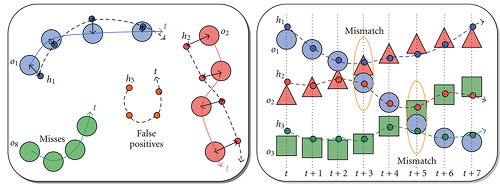
\includegraphics[width=\linewidth]{figs/CLEARMOT_illustration.png} }}%
    \caption{Illustration of the types of errors considered by the CLEAR MOT metrics, courtesy of \cite{CLEARevaluation}.}%
    \label{fig:CLEARMOT_illustration}%
\end{figure}


We used the py-motmetrics library \cite{pymotmetrics}, a popular python library that evaluates multi-object trackers using methods including CLEAR. The outputs of this library are mostly compatible with the MOTChallenge benchmarks. Because the ground truth data and annotations are stored locally, and the tracker runs within a web browser, we developed an evaluation framework in python that interfaces with the web browser; the framework instantiates a web server which requests the tracking results for a provided video. The server then processes these results using py-motmetrics, and also visualizes the tracking results in the form of a gif. The server may also pass parameters to the tracker, which is utilized in the experiments detailed in the experiments section \ref{experiments_section}. This implementation spans about 350 lines of code and can be found in the \texttt{/eval} directory of the project's source code.

In addition to the python evaluation framework, we developed a browser-based demo that captures video from a webcam feed and visualizes the tracking results.
This proved especially helpful in debugging.
This demo can be found at \url{https://julianoks.github.io/670_final_proj/}.




\label{implementation_section}
\section{Implementation}
As described in the Methodology section \ref{methodology_section}, we developed an online tracker that utilizes a MobileNetV2 objection detection model that runs in JavaScript within a web browser.
This section describes how the tracker is implemented and how the computation is executed.
Overall, the tracker runs about 20 frames-per-second, and the implementation spans about 1000 lines of JavaScript code, not including dependencies.
The implementation can be found at \url{https://github.com/julianoks/670_final_proj}.

\label{overview_of_computation}
\subsection{Overview of Computation}
We now describe how the computation is structured into stages.
Please refer back to the Tracking Algorithm \ref{tracking_algo_subsection} for an overview of the computation.
The key to computing these steps efficiently is taking advantage of parallelizability and efficient memory management.

\textbf{Stage 1}
We begin by running two computations in parallel, 1) object detection using the MobilNetV2 model and non-maximum suppression, and 2) calculating the Local Binary Pattern (LBP) code for each pixel.
At this stage, no other computations can be performed as they all depend on the results of the object detector.
We are careful to reuse the same image buffer for both computations, which is the most space-intensive part of the algorithm. The image buffer is discarded once this stage is complete.
On a conventional laptop's web browser, the MobileNetV2 model runs in about 49 milliseconds, and the LBP runs in about 6 milliseconds. 

\textbf{Stage 2}
We now proceed with extracting features for each detection's bounding box.
First, we extract the class features from the model. When running the object detector, we were careful to store this intermediate value.
These values are brought into main memory from the GPU and the intermediate values are flushed.
With the bounding boxes provided by the object detector, we then extract a histogram of the LBP pixel codes for each detection.
For the time being, we aggregate the histograms using a linear scan, which is quite expensive. To mitigate this, we parallelize these aggregations.
However, in the future we'd like to make this aggregation more efficient by using a 2D segment tree data structure which would be constructed in Stage 1.
Although it is slower to build this data structure, because the LBP computation in Stage 1 is non-blocking, building the data structure would not increase Stage 1's running time, but would improve Stage 2's.
Once these aggregations are performed, the LBP code buffer from stage 1 is discarded.

\textbf{Stage 3}
The remainder of the steps (steps 3-6 from \ref{tracking_algo_subsection}) must be performed in series.
These steps were implemented as described, and, for the most part, cannot be optimized much further.


\subsection{Other Implementation Details}
\textbf{The Kalman Filter}
We could not find a suitable implementation of a Kalman Filter, and so we opted to write a Kalman Filter library ourselves, from scratch.
This implementation can be found here: \url{https://gist.github.com/julianoks/4303f4a23ac83c384b890e9afc2a3f52}.

\textbf{The tracker} The tracker was implemented in about 700 lines of modern JavaScript (ES6) code.
An entry point for this code can be found in \texttt{/track.js}, which exposes a "track" class which is used to track (and visualize results) from a webcam feed.
This makes extensive use of the "tracker" class from \texttt{/algorithms/tracker.js}.
Both these scripts use helper functions from \texttt{/algorithms/utils.js}, which contains many extraneous functions that were placed there to make the other classes cleaner.
Many of these functions and methods are documented using JSDoc, however we'd like to fully document every component of the system.

\textbf{MobileNetV2 Object Detector}
We used a quantized MobileNetV2 architecture that was pretrained on the COCO detection dataset.
This model was trained and released by the Tensorflow team. More information about this model can be found \href{https://github.com/tensorflow/models/blob/master/research/slim/nets/mobilenet_v1.md}{here}.
This model was originally built in Python, and was then quantized and ported to tensorflow.js \cite{smilkov2019tensorflowjs}.
A great deal of effort was spent trying to port other models, but this was effort was unsuccessful.

\textbf{Libraries used}
We'd like to thank the authors of the libraries we used,
\begin{itemize}
\item \href{https://www.tensorflow.org/js}{TensorFlow.js} for running the Object Detection model
\item  \href{http://sylvester.jcoglan.com/}{Sylvester} for vector and 2D matrix math
\item \href{https://github.com/ubilabs/kd-tree-javascript}{JavaScript k-d Tree Implementation}
\item \href{https://github.com/mattkrick/hungarian-on3}{Hungarian Algorithm}, which we ported from node.js. We look forward to contributing this port. 
\item \href{http://www.xarg.org/2014/03/javascript-bit-array/}{JavaScript BitSet} implementation, which was used for porting parts of the Hungarian Algorithm. 
\end{itemize}

\label{experiments_section}
\section{Experiments}
After building the system, there were still a number of unresolved questions.
Particularly, we were unsure what the best settings were for our system; different parameters and configurations resulted in very different behaviors.
We directed our efforts towards understanding the effect of our affinity measures, which were described in the Matching Algorithm subsection \ref{matching_algo_subsection}.
We designed a set of experiments to 1) find the best combination of affinity measures to use, and 2) to quantify the benefit of each affinity measure.

\label{optimal_combination_exp}
\subsection{Finding the optimal combination of affinity measures}
In this experiment we were interested in finding the optimal combination of the 4 affinity measures described in subsection \ref{matching_algo_subsection}.
Because there were only 4 measures, we considered the entire power set, which contains only $2^4 = 16$ configurations.
A configuration is any subset of the affinity measures.
The weight function for the empty set configuration was taken to be $w=1$.
For each configuration we evaluated the overall F1 score on the training data, and simply picked the best.
We chose the F1 score because it consider bth the precision and recall of the tracker.
We also felt that, qualitatively, the F1 score appeared to correspond well with what we believed were "good" tracking results.

\label{attribution_experiment}
\subsection{Attributing Utility to Affinity Measures}
Next, we were interested in quantifying the benefit of using each affinity measure.
One method to do so is to consider the change in utility when a measure is removed from the full configuration; i.e. an ablation.
We define utility by the F1 score we described in the previous experiment.
However, the change in utility depends on the configuration used; for example, if there are duplicate affinity measures, removing one from a full configuration may help, but when only one of the duplicates is present, removing it may hurt.
In order to resolve this, we perform an experiment where we calculate the \textit{Shapley Values} \cite{shapley_s_1951} of the affinity measures.

Briefly, the Shapley Values are a means to attribute some cost or utility among a group of agents in a cooperative game.
For the sake of brevity, we omit a detailed explanation of the Shapley Values, but we direct the interested reader to an axiomatic justification \cite{shapley_s_1951}.
In this experiment, we are provided with the utility (F1) score corresponding to every subset of affinity measures.
We calculate the Shapley value of the $i^{th}$ affinity measure as,
$$ \varphi_{i}(v)=\sum_{S \subseteq N \backslash\{i\}} \frac{|S| !(N-|S|-1) !}{N !}(v(S \cup\{i\})-v(S)) $$
where $N=4$ is the number of affinity measures, $S$ is any configuration (a subset), and $v$ is a function that gives the F1 score of a configuration.

\subsection{A/B Tests}
One area of focus was the parameters and thresholds defined in the Matching Algorithm subsection \ref{matching_algo_subsection}.
Initially, these were chosen somewhat arbitrarily.
We deemed that jointly optimizing these parameters in a systematic way would require a lot of effort of computing power, and so we instead optimized them in an ad-hoc fashion, manually conducting A/B tests over the training data.
This certainly improved the tracker, however we did not record the A/B tests because it was a more informal part of the development process.
In the future we'd like to give a more rigorous characterization of the effects of these parameters.


\label{results_section}
\section{Results}
In this section we describe the results of our experiments \ref{experiments_section}, as well as the overall results on the 2015 MOTChallenge \cite{motchallenge2015} dataset.

\textit{Note:} As mentioned in \ref{greedy_vs_hungarian}, there were issues with the Hungarian Algorithm implementation that caused it to crash on certain inputs; for this reason, we developed a (suboptimal) greedy algorithm.
Because some experiments encountered a large set of inputs that caused the Hungarian Algorithm to crash, we sometimes had to use the suboptimal greedy algorithm.
We make explicit which results used the greedy or the Hungarian algorithm.
 
\subsection{Combination of Affinity Measures}
\textit{Note: These results were obtained using the greedy matching algorithm.}

We evaluated the performance of every combination of affinity measure, as described in \ref{optimal_combination_exp}.
Table \ref{tab:f1_scores_configs} shows these results.
We found that the optimal combination used the "MobilNetV2 Class Distribution" and "Intersection-Over-Union" affinity measures \ref{matching_algo_subsection}, but not the "Local Binary Pattern" or "Kalman Transition Probability" measures.
On the training set, this combination received an overall F1 score of 66.5.

However, we have reason to doubt these results.
The first reason is that the F1 score for this configuration with the "Kalman Transition Probability" affinity measure was rather close, achieving an F1 score of 62.8.
We believe the Kalman measure is helpful for disambiguations in scenarios where, for example, two people cross paths. The greedy matching algorithm seems to behave unpredictable in these scenarios. 
Thus we believe we may get slightly different results if we were to use the Hungarian algorithm.
We were able to use the Hungarian algorithm on a configuration with the \{"MobilNetV2 Class Distribution", "Intersection-Over-Union"\} and \{"MobilNetV2 Class Distribution", "Intersection-Over-Union", "Kalman Transition Probability"\}, and we actually found that including the Kalman affinity measure improved our results.
The final reason we believe the result was skewed by the use of the greedy algorithm was that the attribution experiment \ref{attribution_experiment} suggests the Kalman affinity measure is beneficial.
\begin{table}[h]
\begin{tabular}{|l|l|l|l|l|}
\hline
Class Feature & IOU        & Kalman     & LBP        & F1 Score \\ \hline
\checkmark    & \checkmark &            &            & 66.5     \\ \hline
\checkmark    &            &            &            & 64.2     \\ \hline
\checkmark    &            & \checkmark &            & 63.3     \\ \hline
              &            & \checkmark &            & 62.8     \\ \hline
\checkmark    & \checkmark & \checkmark &            & 62.8     \\ \hline
              & \checkmark & \checkmark &            & 62.3     \\ \hline
              & \checkmark &            &            & 60.5     \\ \hline
              &            &            &            & 47.6     \\ \hline
\checkmark    &            & \checkmark & \checkmark & 40.3     \\ \hline
              &            & \checkmark & \checkmark & 40.1     \\ \hline
\checkmark    &            &            & \checkmark & 37.1     \\ \hline
\checkmark    & \checkmark & \checkmark & \checkmark & 37.0     \\ \hline
              & \checkmark & \checkmark & \checkmark & 36.7     \\ \hline
              &            &            & \checkmark & 36.2     \\ \hline
\checkmark    & \checkmark &            & \checkmark & 24.2     \\ \hline
              & \checkmark &            & \checkmark & 23.9     \\ \hline
\end{tabular}
\caption{F1 score of each configuration.}
\label{tab:f1_scores_configs}
\end{table}


\begin{table}[h]
\begin {center}
\begin{tabular}{|l|l|}
\hline
\textbf{Affinity Measure} & \textbf{Shapley Value} \\ \hline
Intersection Over Union   & 0.125                  \\ \hline
Local Binary Pattern      & -24.075                \\ \hline
Class Distribution        & 4.925                  \\ \hline
Kalman Probability        & 8.425                  \\ \hline
\end{tabular}
\caption{Shapley value of each affinity measure.}
\label{tab:shapley_val_table}
\end{center}
\end{table}


\begin{figure*}[h]
\begin{verbatim}
                IDF1   IDP    IDR   Rcll  Prcn  GT  MT PT ML    FP   FN IDs  FM   MOTA  MOTP
TUD-Stadtmitte 85.6% 95.0%  77.9%  80.9% 98.7%  10   7  3  0    12  221   4   4  79.5% 0.703
ETH-Bahnhof    64.9% 52.2%  86.0%  99.0% 60.0% 223 214  7  2  5057   78  84   3  32.0% 0.884
TUD-Campus     86.7% 76.5% 100.0% 100.0% 76.5%   8   8  0  0   110    0   4   0  68.2% 0.773
ETH-Sunnyday   65.1% 52.4%  86.0%  99.7% 60.7%  30  30  0  0  1227    5  18   0  34.2% 0.849
ADL-Rundle-8   64.2% 55.7%  75.7%  99.3% 73.1%  28  28  0  0  2481   50  52   2  61.9% 0.937
KITTI-17       67.2% 57.9%  80.1%  83.6% 60.4%   9   5  4  0   428  128   5   0  28.3% 0.858
ETH-Pedcross2  72.7% 78.2%  68.0%  80.2% 92.2% 151  92 30 29   460 1336  81  49  72.2% 0.810
KITTI-13       47.6% 32.6%  87.9%  97.8% 36.3%  42  41  1  0  1596   20  22   3  76.3% 0.939
ADL-Rundle-6   75.3% 81.4%  70.0%  84.4% 98.1%  24  16  8  0    80  783  30  24  82.2% 0.861
Venice-2       73.9% 67.5%  81.5%  99.5% 82.3%  26  26  0  0  1525   39  38   3  77.6% 0.925
PETS09-S2L1    55.9% 45.8%  71.6% 100.0% 64.0%  19  19  0  0  2618    0  60   0  42.4% 0.784
OVERALL        67.2% 59.4%  77.3%  93.8% 72.2% 570 486 53 31 15594 2660 398  88  56.8% 0.870
\end{verbatim}
\caption{Results on the 2015 MOTChallenge dataset \cite{motchallenge2015}. See \href{https://github.com/cheind/py-motmetrics/blob/master/Readme.md\#metrics}{here} for a description of the columns.}
\label{tab:MOT_results}
\end{figure*}



\begin{figure*}[h]
    \centering
    \subfloat[t=3]{{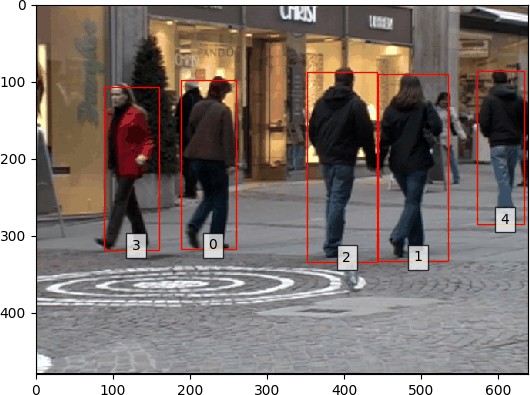
\includegraphics[width=0.15\linewidth]{./figs/example_frames/TUD-Stadtmitte-3.png} }}%
    \subfloat[t=5]{{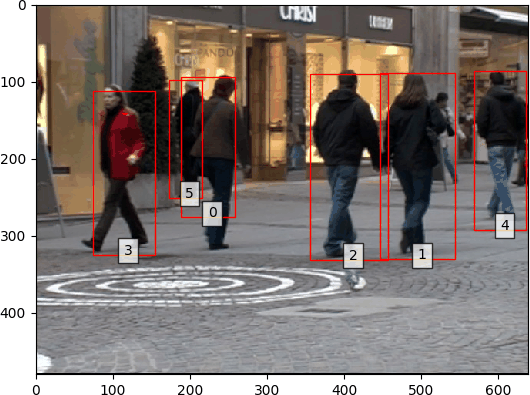
\includegraphics[width=0.15\linewidth]{./figs/example_frames/TUD-Stadtmitte-5.png} }}%
    \subfloat[t=13]{{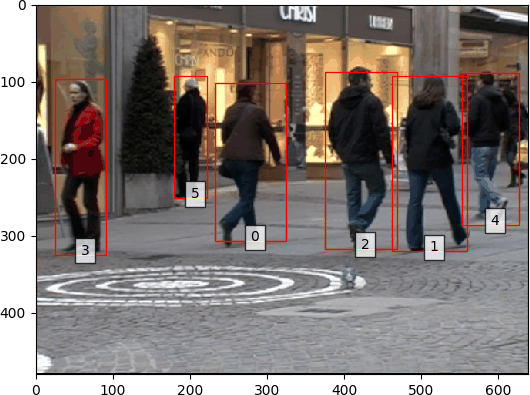
\includegraphics[width=0.15\linewidth]{./figs/example_frames/TUD-Stadtmitte-13.png} }}%
    \subfloat[t=18]{{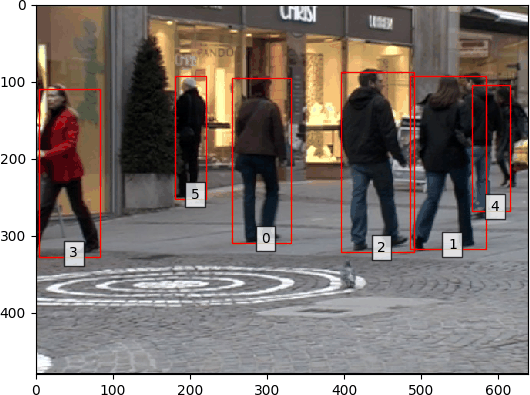
\includegraphics[width=0.15\linewidth]{./figs/example_frames/TUD-Stadtmitte-18.png} }}%
    \subfloat[t=24]{{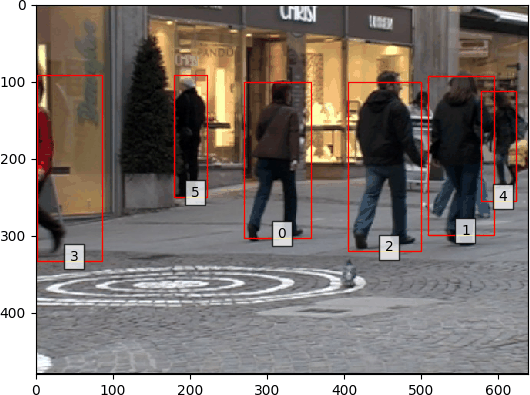
\includegraphics[width=0.15\linewidth]{./figs/example_frames/TUD-Stadtmitte-24.png} }}%
    \subfloat[t=33]{{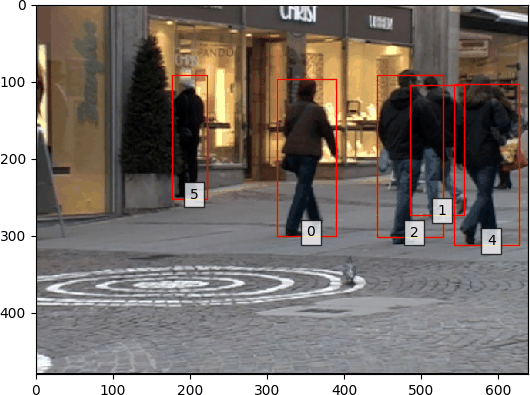
\includegraphics[width=0.15\linewidth]{./figs/example_frames/TUD-Stadtmitte-33.png} }}%
    \caption{Tracking results on the TUD-Stadtmitte video.}
    \label{fig:example_frame_train}%
\end{figure*}


\subsection{Attributing Utility to Affinity Measures}
\textit{Note: These results were obtained using the greedy matching algorithm.}

From the results presented in \ref{tab:f1_scores_configs}, we calculated the Shapley value of each affinity measure, which is displayed in table \ref{tab:shapley_val_table}.
These values are consistent with our observations; for example, the Local Binary Pattern affinity measure hurts all configurations it is added to, and thus it has a strongly negative Shapley value.
The Shapley values for the remaining affinity measures suggest that adding these generally has a positive effect.





\subsection{Results on 2015 MOTChallenge Dataset}
\textit{Note: These results were obtained using the Hungarian matching algorithm.}


Table \ref{tab:MOT_results} shows the results on the 2015 MOTChallenge dataset \cite{motchallenge2015}, evaluated using the py-motmetrics library \cite{pymotmetrics}.
These results are extremely competitive with the 2015 leaderboard (\url{https://motchallenge.net/results/2D_MOT_2015/?chl=2}) on most metrics.
One reason our results may be so competitive is because we use a high-quality Object Detection model from 2019, whose quality far exceeds what was available in 2015. 
The results from the 2017 leaderboard (\url{https://motchallenge.net/results/MOT17Det/}) mostly used different metrics, but the results seemed better than those from 2015 and the results we obtained.
Something to note is that the leaderboard's results are evaluated on the challenge's testing data, whose ground-truth annotations are kept private, whereas our results are derived from the challenge's training data.
Figure \ref{fig:example_frame_train} shows an example of tracking results on the TUD-Stadtmitte video.



\label{time_and_space_eff}
\subsection{Time and Space Efficiency}
As described in subsection \ref{overview_of_computation}, we decomposed our computation into 3 stages.
Using the \href{https://developers.google.com/web/updates/2016/12/devtools-javascript-cpu-profile-migration}{Chrome JavaScript Profiler}, we analyzed the runtime performance of each stage.
We measured this on a conventional laptop's Chrome Browser.
We found that stage 1 runs in 49 milliseconds; 49 milliseconds are needed for the Object Detection model, and 6 milliseconds are needed for calculating the Local Binary Pattern codes.
Because these computations are run in parallel, stage 1 takes a total of 49 milliseconds.
Together, stages 2 and 3 require just under 1 millisecond.
Altogether, our system runs in 50 milliseconds, which is 20 frames per second.

Using the MobileNetV2 Object Detector, this is a near-optimal runtime.
98\% of this time is devoted to the Object Detection Model; if we'd like a faster tracker, we'd need a faster Object Detection model.

The system requires about 20 megabytes of memory, which we'd consider to be very lightweight.
Similar to the tracker's runtime, virtually all the memory consumption comes from the Object Detection model.
If one would like a more memory efficient tracker, we'd need a more memory efficient Object Detection model.

\section{Discussion and Future Work}
\label{assumptions_discussion}
\subsection{Assumptions}
\textbf{Static Camera and Small Motion Assumptions}. 
These assumptions are essential to our motion model and matching algorithm.
In many ways, these are similar assumptions; the camera captures the relative motion, which is assumed to be gradual.
The k Nearest Neighbors component of the matching algorithm assumes that the projection of an object's center does not move very much between frames.
Likewise, the intersection-over-union affinity measure relies on these assumptions, as well as the the Kalman Filter.
In every case we've seen, the small motion assumptions holds, however the static camera assumption does not always hold.
However, the algorithm seems to tolerate a small amount of camera motion, as long as it is gradual; an object's projection is still relatively consistent over time.
However, when the algorithm encountered video from a rapidly-moving camera (filmed from a train), the algorithm failed.

\textbf{Consistent Appearance}
The matching algorithm's use of appearance-based affinity measures assumes that an object's appearance is consistent over time (or may change slowly, hence the exponential moving average).
This assumptions seems to be beneficial if the method of measuring similarity is effective; the class feature was highly beneficial whereas the Local Binary Pattern feature was detrimental.
One explanation for this is that the class distribution may be more consistent between frames, whereas the local binary pattern may fluctuate a lot, due to changes in viewpoint, occlusions, etc.

\textbf{Consistent Velocity} - This assumption is used by the Kalman Filter (see implementation), which is used as both an affinity measure (ie how likely is this movement?), as well as being used to propagate lost objects by updating their position (with an estimate of their velocities).
There are plenty of scenarios where this assumption does not hold; objects change trajectory, stop, and perspective projection may changes the apparent velocity.
Although the Kalman affinity measure seems to work well, we cannot give any conclusive results about this assumption.


\textbf{Consistent Size} - This assumption is used by intersection-over-union affinity measure.
It seems to generally hold, except in the case where an object moves towards or away from the camera, however the change in size is very gradual, and the algorithm seems to tolerate this well.


\subsection{Implementation}
One especially important issue that remains partially unresolved is the instability of our Hungarian algorithm, which negatively impacted some of our results.
Our implementation is fairly well documented, however we'd like to more extensively document the system and expose a greater variety of interfaces.
We used a number of JavaScript libraries that do not have licenses, and so we'd like to authorize the use of these libraries before distributing the system.
Otherwise, the implementation is fairly complete, and as discussed in subsection \ref{time_and_space_eff}, there is not much room for efficiency optimizations, besides using a different object detector.


\section{Conclusion}
In this report we described a multi-object tracker that was designed to operate in real-time within a web browser.
Our analysis showed that we successfully developed a very efficient lightweight tracker that is capable of running 20 frames per second with minimal memory consumption.
We developed a tracking algorithm which works fairly well.
We analyzed some components of the tracking algorithm, particularly the affinity measures, and found that certain motion and appearance related measures were beneficial, while some measures, particularly the Local Binary Pattern measure, hurt performance.
We used the findings of our experiments to fine-tune our tracking algorithm, ultimately receiving a very respectable F1 score of 67.2\%.

Implementing this project in the browser was a massive engineering effort.
Throughout the report we mentioned several implementation challenges that we overcame, and some that we did not.
Nonetheless, we are proud to have developed such a novel application in spite of these challenges.



{\small
\bibliographystyle{ieee_fullname}
\bibliography{report}
}

\end{document}
